\documentclass[11pt]{article}
\usepackage{geometry}
\geometry{letterpaper}

\usepackage{graphicx}
\usepackage{amssymb}
\usepackage{float}
\usepackage{tabularx}
\usepackage{multicol}
\usepackage{hyperref}
\hypersetup{
    colorlinks,
    citecolor=black,
    filecolor=blue,
    linkcolor=black,
    urlcolor=black
}

% TODOs:
% ask Nick about lines in Seq Diagram, ask Nick about need 3D model, ask Nick about entering project goals
% switch to cleveref

\begin{document}

\begin{titlepage}
	\newcommand{\HRule}{\rule{\linewidth}{0.2mm}}
	\begin{center}
	\textsc{\LARGE McMaster University}\\[1.5cm]

	\textsc{\Large SmartServe}\\[0.5cm]
	\textsc{\large Software \& Mechatronics Capstone}\\[0.5cm]

	\HRule\\[0.4cm]
		{\huge\bfseries Hazard Analysis}\\[0.4cm]
	\HRule\\[0.4cm]

	\begin{minipage}[t][][t]{0.5\textwidth}
		\begin{flushleft} \large
			\emph{Authors:}\\
			Christopher McDonald\\
			Harit Patel \\
			Janak Patel \\
			Jared Rayner  \\
			Nisarg Patel  \\
			Sam Hamel \\
			Sharon Platkin \\
		\end{flushleft}
	\end{minipage}
	~
	\begin{minipage}[t][][t]{0.4\textwidth}
		\begin{flushright} \large
			\emph{Professor:} \\
			Dr. Alan Wassyng \\[0.4cm]
			\emph{Teaching Assistants:} \\
			Bennett Mackenzie \\
			Nicholas Annable \\
			Stephen Wynn-Williams \\
			Viktor Smirnov
		\end{flushright}
	\end{minipage}\\[2cm]

	
\includegraphics[width=0.3\textwidth]{logo.png} \\
	{\large Last compiled on \today}
	\end{center}

\end{titlepage}

\tableofcontents
\listoffigures

\vfill
\begin{figure}[H]
   \centering
   \noindent\begin{tabularx}{\textwidth}{| >{\centering\arraybackslash}m{0.2\textwidth} | >{\centering\arraybackslash}m{0.2\textwidth} | >{\centering\arraybackslash}m{0.2\textwidth} | >{\centering\arraybackslash}m{0.285\textwidth} |}
   \hline
   \textbf{Date} & \textbf{Revision} & \textbf{Comments} & \textbf{Author(s)} \\ \hline
   Dec 29, 2017 & 1.0 & Main content done for all sections & Christopher McDonald \\ \hline
   Jan 1, 2018 & 2.0 & Edit entire document & Sharon Platkin \\ \hline
   \end{tabularx}
   \caption{Revision History}
\end{figure}
\newpage
\section{Introduction}
\subsection{Project Overview}
SmartServe is an autonomous table tennis training system for table tennis players with various skill levels. SmartServe aids in diagnosing and improving a player's performance over time. The system trains table tennis players by shooting table tennis balls towards the player and detects successful returns from the player. The system can further adapt to the player's weaknesses and help them overcome it through further training. Importantly, SmartServe alleviates the problems of finding and working with a coach for players, as well as coaches trying to train multiple players simultaneously. The system will be deemed a success if the table tennis players and coaches can enjoy and see some value added by using SmartServe.\\ \\
The project started at the beginning of the Fall 2017 academic term and will conclude at the end of the Winter 2018 term. In addition, the core project team consists of final year Software and Mechatronics Engineering students who are enrolled in the MECHTRON 4TB6/SFWRENG 4G06 capstone project course.
\subsection{Document Overview}
This document will cover all potential hazards that a user may encounter when using the SmartServe system. For each hazard, a description, mitigation plan, and a fault tree to cover all potential situations in which the hazard would arise are included. Additionally, a description of the system, its scope, and boundary will be provided in order to support and provide context to the hazards.
\subsection{Naming Conventions and Terminology}
\label{sec:definitions}
The following terms and definitions will be used throughout this document:
\begin{itemize}
\item \textbf{ACID}: a database transaction which is atomic, consistent, isolated and durable
\item \textbf{CV}: computer vision
\item \textbf{FPS}: frames per second
\item \textbf{FSM}: finite state machine, shows transitions between states
\item \textbf{GUI}: graphical user interface
\item \textbf{IPO}: input process output
\item \textbf{ITTF}: International Table Tennis Federation
\item \textbf{Pitch}: rotation along the y-axis; this rotation angle primarily dictates the range of the ball from the net to the edge of the table on the user side
\item \textbf{Roll}: rotation along the x-axis
\item \textbf{Shooting Mechanism}: refers to the part of the system that shoots the table tennis balls towards the user side (player) Please refer to Figure \ref{fig:table-tennis-top-view} for visual illustration
\item \textbf{System}: encompasses both the hardware and software parts of SmartServe
\item \textbf{System Side}: the side of the table where the electromechanical system is placed; it is the opposite side of the User Side Please refer to Figure \ref{fig:table-tennis-top-view} for visual illustration
\item \textbf{TCP:} transmission control protocol
\item \textbf{Team}: all team members of the core capstone project, as noted in the list of Authors
\item \textbf{User Side}: the side of the table where the user (player) is standing
\item \textbf{Yaw}: rotation along the z-axis; this rotation angle primarily dictates the panning functionality of the shooting mechanism from the right side to the left side of the table
\end{itemize}

\begin{figure}[H]
   \centering
   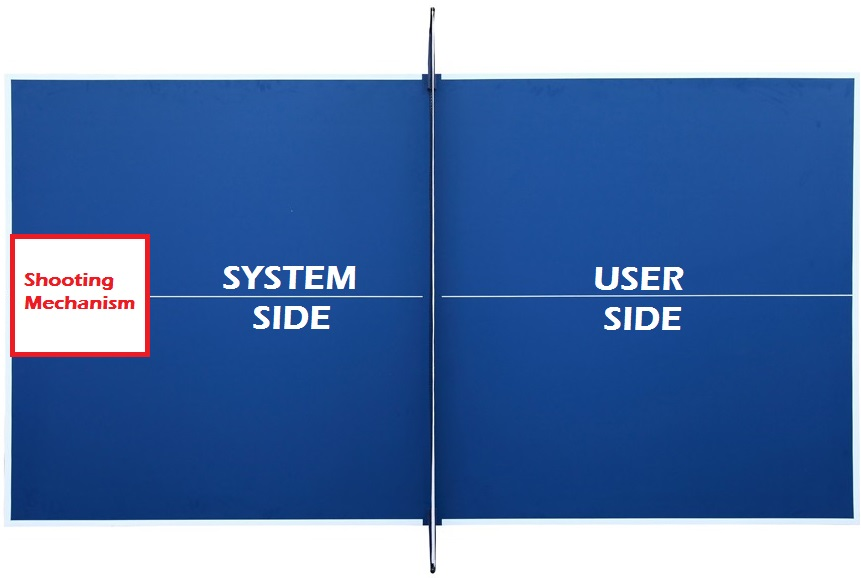
\includegraphics[width=0.75\textwidth]{img/Table-Tennis-Top-View.png}
   \caption{Top View of the Tennis Table}
   \label{fig:table-tennis-top-view}
\end{figure}

\section{System}
\subsection{High-Level Design}
The high-level design document covers in great detail the design of the system and can be found \href{run:../SystemDesign/Design.pdf}{here}. As a summary, the mechanical aspects include a hopper to hold all the table tennis balls and a spinning disk with cut outs to force feed the balls into the barrel. The barrel can hold many balls and they are pushed up the barrel as the aforementioned disk spins. Once a ball reaches the end of the barrel, it will shoot the ball out via a spinning wheel affixed to the end of the barrel. The entire mechanism is fixed to a rotating platform to have variable yaw. The spinning wheel can shoot at various speeds. \\ \\
The electrical components include an Arduino, breadboard and power supply to control the motors needed to spin the mechanism and wheel. There will also be a general purpose computer to run the software-based components and a USB camera to use for the computer vision system. 
\subsection{Scope \& Boundary}
The hazards outlined below will cover the hardware, electrical and software aspects of the SmartServe system. \\ \\
Intentional misuse or destruction of the system will not be discussed as it is outside the scope of this document. The user is assumed to be using fully-functioning and maintained equipment including the table tennis balls, table and paddles. All electrical equipment is assumed to be working at production performance which includes all electrical wiring, components, boards and motors.   
\section{Hazards}
\subsection{User is struck by an air-borne ball}
\subsubsection*{Description}
The machine will be shooting balls towards the user for them to return. For normal shots, it should always hit the table on the user side first before hitting a player. Not only is this a rule for valid shots as per the International Table Tennis Federation(ITTF) rules, it will ensure a sufficient amount of time for the user to react. However, the system could shoot the ball directly towards the player without hitting the table. This could potentially cause damage to the face or eyes of the player if the ball is travelling fast enough.
\subsubsection*{Mitigation Plan}
The system should never attempt to take a shot which exceeds the length of the user's side of the table. However, if a user were to replace the table with a smaller one without calibration or if some bug does make the spinning wheel spin faster than allowed, this could happen. The motor for the spinning wheel should have a maximum voltage in order to ensure the ball isn't shot at high speeds which would cause damage. \\ \\
The fault analysis tree can be found in Figure \ref{fig:ft-Air}.
\begin{figure}[H]
   \centering
   \includegraphics[width=0.7\textwidth]{img/ft-Air.png} % requires the graphicx package
   \caption{Fault Analysis Tree for \textit{User is struck by an air-borne ball}}
   \label{fig:ft-Air} %TODO: ITTFF should be ITTF
\end{figure}

\subsection{User is caught in a Pinch Point}
\subsubsection*{Description}
The system will include moving mechanisms to shoot balls toward the player in a variety of ways. This means that two pieces could be moving next to one another. This may lead to a user's finge or other extremity being caught in between the two pieces. This can cause damage to the user and the system. The system can break the users skin or bones and the motors and materials can break if given enough force.
\subsubsection*{Mitigation Plan}
The number of pinch points should be minimized in order to avoid the chance of this happening. In the event one is unable to be avoided, proper notices and warnings will be used to discourage accidental exposure of the user's extremeties to the pinch points. Additionally, guards will be installed wherever possible. \\ \\
The fault analysis tree can be found in Figure \ref{fig:ft-pinch}.

\begin{figure}[H]
   \centering
   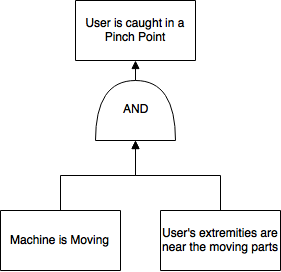
\includegraphics[width=0.7\textwidth]{img/ft-pinch.png} % requires the graphicx package
   \caption{Fault Analysis Tree for \textit{User is caught in a Pinch Point}}
   \label{fig:ft-pinch}
\end{figure}

\subsection{Electric Shock}
\subsubsection*{Description}
The system will require electrical components in order to activate motors. This will also include power balancing and transfer to the necessary components. This means some wiring will be needed and thus some inherent risk of shock to the user via such wiring or the sensors or actuators themselves. Only when the wires carry current would this be a risk.
\subsubsection*{Mitigation Plan}
All wiring will be enclosed to the best of our ability. However, due to the nature of the system requiring motion it can be difficult to completely enclose the system. Proper warnings and notices will be used to warn the user of electrical current. The system will also be fused to prevent prolonged short circuits. \\ \\

The fault analysis tree can be found in Figure \ref{fig:ft-electric}.

\begin{figure}[H]
   \centering
   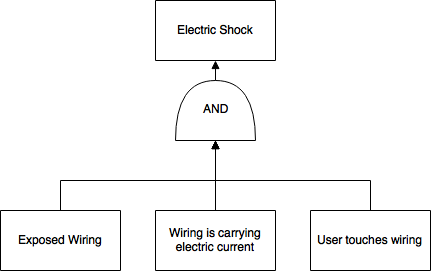
\includegraphics[width=0.7\textwidth]{img/ft-electric.png} % requires the graphicx package
   \caption{Fault Analysis Tree for \textit{Electric Shock}}
   \label{fig:ft-electric}
\end{figure}

\subsection{User's appendage is caught in machine}
\subsubsection*{Description}
Similar to a user's extremity, any loose appendages can also be of risk due to moving parts. An appendage could be a necklace, bracelet or any accessory. The risk goes up substantially for loose appendages. When the machine is moving, the appendage could get caught on or in between moving parts. When caught it could damage the appendage, the machine or the user.
\subsubsection*{Mitigation Plan}
The user must be warned not to wear such appendages when using this system. The number of points which would be vulnerable should be minimized. Similar to the extremity hazard, the locations which are vulnerable will be labelled appropriately and guarded. \\ \\

The fault analysis tree can be found in Figure \ref{fig:ft-appendage}.

\begin{figure}[H]
   \centering
   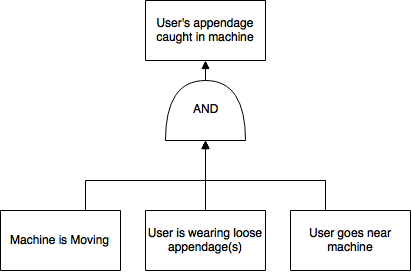
\includegraphics[width=0.7\textwidth]{img/ft-appendage.png} % requires the graphicx package
   \caption{Fault Analysis Tree for \textit{User's appendage is caught in machine}}
   \label{fig:ft-appendage}
\end{figure}

\subsection{Machine overheats}
\subsubsection*{Description}
The system is vulnerable to friction and overheating via electricity. This could cause mechanical failure where parts are damaged by this heat. It could also cause burns for a user who tries to handle the system when it overheats.
\subsubsection*{Mitigation Plan}
The system should shutdown after extreme prolonged use and is designed with appropriate fusing such that the power supply never exceeds electric load. \\ \\

The fault analysis tree can be found in Figure \ref{fig:ft-overheat}.

\begin{figure}[H]
   \centering
   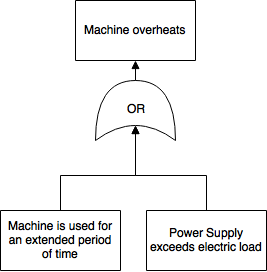
\includegraphics[width=0.7\textwidth]{img/ft-overheat.png} % requires the graphicx package
   \caption{Fault Analysis Tree for \textit{Machine overheats}}
   \label{fig:ft-overheat}
\end{figure}

\subsection{Machine's traversal is blocked}
\subsubsection*{Description}
As stated before, the system will contain moving parts to shoot in a variety of ways. A foreign object could be in the path which the system needs to travel. The system will attempt to travel this distance and if the foreign object isn't moved, either by the user or the machine itself, it could cause damage to the motors and mechanical parts of the system.
\subsubsection*{Mitigation Plan}
The user should ensure the system is clear of foreign objects within a certain radius of the machine and will be reminded to do so upon booting up the system. \\ \\

The fault analysis tree can be found in Figure \ref{fig:ft-traverse}.

\begin{figure}[H]
   \centering
   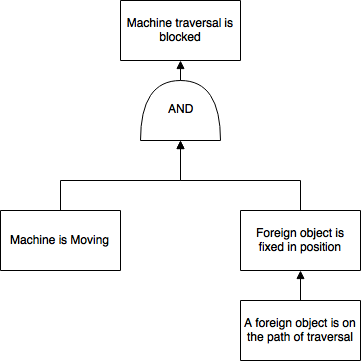
\includegraphics[width=0.7\textwidth]{img/ft-traverse.png} % requires the graphicx package
   \caption{Fault Analysis Tree for \textit{Machine's traversal is blocked}}
   \label{fig:ft-traverse}
\end{figure}

\end{document}
